\documentclass[a4paper,12pt]{article}
\usepackage[top = 2.5cm, bottom = 2.5cm, left = 2.5cm, right = 2.5cm]{geometry}
\usepackage[T1]{fontenc}
\usepackage[utf8]{inputenc}
\usepackage{multirow} 
\usepackage{booktabs} 
\usepackage{graphicx}
\usepackage[spanish]{babel}
\usepackage{setspace}
\setlength{\parindent}{0in}
\usepackage{float}
\usepackage{fancyhdr}
\usepackage{amsmath}
\usepackage{amssymb}
\usepackage{amsthm}
\usepackage[numbers]{natbib}
\newcommand\Mycite[1]{%
	\citeauthor{#1}~[\citeyear{#1}]}
\usepackage{graphicx}
\usepackage{subcaption}
\usepackage{booktabs}
\usepackage{etoolbox}
\usepackage{minibox}
\usepackage{hyperref}
\usepackage{xcolor}
\usepackage[skins]{tcolorbox}
%---------------------------

\newtcolorbox{cajita}[1][]{
	 #1
}

\newenvironment{sol}
{\renewcommand\qedsymbol{$\square$}\begin{proof}[\textbf{Solución.}]}
	{\end{proof}}

\newenvironment{dem}
{\renewcommand\qedsymbol{$\blacksquare$}\begin{proof}[\textbf{Demostración.}]}
	{\end{proof}}

\newtheorem{problema}{Problema}
\newtheorem{definicion}{Definición}
\newtheorem{ejemplo}{Ejemplo}
\newtheorem{teorema}{Teorema}
\newtheorem{corolario}{Corolario}[teorema]
\newtheorem{lema}[teorema]{Lema}
\newtheorem{prop}{Proposición}
\newtheorem*{nota}{\textbf{NOTA}}
\renewcommand\qedsymbol{$\blacksquare$}
\usepackage{svg}
\usepackage{pgfplots}
\pgfplotsset{compat=1.11}

\usepackage{tikz}
\usetikzlibrary{calc}

\usetikzlibrary{patterns}
\usepackage[framemethod=default]{mdframed}
\global\mdfdefinestyle{exampledefault}{%
linecolor=lightgray,linewidth=1pt,%
leftmargin=1cm,rightmargin=1cm,
}




\newenvironment{noter}[1]{%
\mdfsetup{%
frametitle={\tikz\node[fill=white,rectangle,inner sep=0pt,outer sep=0pt]{#1};},
frametitleaboveskip=-0.5\ht\strutbox,
frametitlealignment=\raggedright
}%
\begin{mdframed}[style=exampledefault]
}{\end{mdframed}}
\newcommand{\linea}{\noindent\rule{\textwidth}{3pt}}
\newcommand{\linita}{\noindent\rule{\textwidth}{1pt}}

\AtBeginEnvironment{align}{\setcounter{equation}{0}}
\pagestyle{fancy}

\fancyhf{}









%----------------------------------------------------------
\lhead{\footnotesize Geometría diferencial}
\rhead{\footnotesize  Rudik Roberto Rompich}
\cfoot{\footnotesize \thepage}


%--------------------------

\begin{document}
 \thispagestyle{empty} 
    \begin{tabular}{p{15.5cm}}
    \begin{tabbing}
    \textbf{Universidad del Valle de Guatemala} \\
    Departamento de Matemática\\
    Licenciatura en Matemática Aplicada\\\\
   \textbf{Estudiante:} Rudik Roberto Rompich\\
   \textbf{Correo:}  \href{mailto:rom19857@uvg.edu.gt}{rom19857@uvg.edu.gt}\\
   \textbf{Carné:} 19857
    \end{tabbing}
    \begin{center}
        Geometría diferencial - Catedrático: Alan Reyes\\
        \today
    \end{center}\\
    \hline
    \\
    \end{tabular} 
    \vspace*{0.3cm} 
    \begin{center} 
    {\Large \bf  Tarea
} 
        \vspace{2mm}
    \end{center}
    \vspace{0.4cm}
%--------------------------


\begin{problema}


$$
\begin{aligned}
& \mathbf{A}=2 \mathbf{a}_{x}+\mathbf{a}_{y}-3 \mathbf{a}_{z} \\
& \mathbf{B}=\mathbf{a}_{y}-\mathbf{a}_{z} \\
& \mathbf{C}=3 \mathbf{a}_{x}+5 \mathbf{a}_{y}+7 \mathbf{a}_{z}
\end{aligned}
$$

Determinar:

\begin{enumerate}
    \item $\mathrm{A}-2 \mathrm{~B}+\mathrm{C}$
    \begin{sol}
        Sea 
        \begin{align*}
            \mathrm{A}-2 \mathrm{~B}+\mathrm{C} &= (2,1,-3) -2\cdot (0,1,-1)+(3,5,7)\\
            &= (2,1,-3) - (0,2,-2)+(3,5,7)\\
            &= (2,-1,-1) +(3,5,7)\\
            &= (5,4,6)\\
        \end{align*}
    \end{sol}

    \item $\mathrm{C}-4(\mathrm{A}+\mathrm{B})$
    \begin{sol}
        Sea 
        \begin{align*}
            \mathrm{C}-4(\mathrm{A}+\mathrm{B}) &=(3,5,7)-4((2,1,-3)+(0,1,-1))\\
            &= (3,5,7)-4(2,2,-4)\\
            &= (3,5,7)-(8,8,-16)\\
            &= (-5,-3,23)\\
        \end{align*}
    \end{sol}
    \item $\frac{2 \mathrm{A}-3 \mathrm{B}}{|\mathrm{C}|}$

    \begin{sol}
        Sea
        \begin{align*}
            \frac{2 \mathrm{A}-3 \mathrm{B}}{|\mathrm{C}|} &=\frac{2(2,1,-3)-3(0,1,-1)}{|(3,5,7)|}\\
            &= \frac{(4,2,-6)-(0,3,-3)}{\sqrt{3^2+5^2+7^2}}\\
            &= \frac{(4,-1,-3)}{\sqrt{9+25+49}}\\
            &= \frac{(4,-1,-3)}{\sqrt{83}}\\
        \end{align*}
    \end{sol}

    
    \item $\mathrm{A} \cdot \mathrm{C}-|\mathrm{B}|^{2}$
    \begin{sol}
        Sea
        \begin{align*}
            \mathrm{A} \cdot \mathrm{C}-|\mathrm{B}|^{2}  &= (2,1,-3)\cdot(3,5,7)-(0,1,-1)\cdot(0,1,-1)\\
            &= 2*3+1*5-3*7 - (0*0+1*1+(-1)*(-1))\\
            &= 6+5-21-(0+1+1)\\
            &= -10-2\\
            &= -12
        \end{align*}
    \end{sol}

    \item $\frac{1}{2} \mathrm{B} \times\left(\frac{1}{3} \mathrm{A}+\frac{1}{4} \mathrm{C}\right)$
    \begin{sol}
        Sea
        \begin{align*}
            \frac{1}{2} \mathrm{B} \times\left(\frac{1}{3} \mathrm{A}+\frac{1}{4} \mathrm{C}\right)  &= \frac{1}{2}\left(0,1,-1\right)\times \left(\frac{1}{3} (2,1,-3)+\frac{1}{4}(3,5,7)\right)\\
            &= \frac{1}{2}\left(0,1,-1\right)\times \left(\frac{2}{3}+\frac{3}{4},\frac{1}{3}+\frac{5}{4},\frac{-3}{3}+\frac{7}{4}\right)\\
            &= \frac{1}{2}\left(0,1,-1\right)\times \left(\frac{2}{3}+\frac{3}{4},\frac{1}{3}+\frac{5}{4},\frac{-3}{3}+\frac{7}{4}\right)\\
            &= \frac{1}{2}\left(0,1,-1\right)\times \left(\frac{15}{12},\frac{19}{12},\frac{-3}{4}\right)\\
            &= \frac{1}{2}\left(\frac{-3}{4}+\frac{19}{12},\frac{15}{12},\frac{15}{12}\right)\\
            &= \frac{1}{2}\left(\frac{10}{12},\frac{15}{12},\frac{15}{12}\right)\\
            &= \left(\frac{10}{24},\frac{15}{24},\frac{15}{24}\right)\\
        \end{align*}
    \end{sol}
\end{enumerate}

\end{problema}

\begin{problema}
Given that

$$
\begin{aligned}
& \mathbf{P}=2 \mathbf{a}_{x}-\mathbf{a}_{y}-2 \mathbf{a}_{z} = (2,-1,-2) \\
& \mathbf{Q}=4 \mathbf{a}_{x}+3 \mathbf{a}_{y}+2 \mathbf{a}_{z} = (4,3,2)\\
& \mathbf{R}=-\mathbf{a}_{x}+\mathbf{a}_{y}+2 \mathbf{a}_{z} = (-1,1,2)
\end{aligned}
$$

Find:
\begin{enumerate}
    \item $|\mathbf{P}+\mathbf{Q}-\mathbf{R}|$
    \begin{sol}
        Sea 
        \begin{align*}
            |\mathbf{P}+\mathbf{Q}-\mathbf{R}| &= |(2,-1,-2)+(4,3,2)-(-1,1,2)|\\
            &= |(7,1,-2)|\\
            &= \sqrt{7^2+1^2+2^2}\\
            &= \sqrt{54}
        \end{align*}
    \end{sol}
    \item $\mathbf{P} \cdot \mathbf{Q} \times \mathbf{R}$
    \begin{sol}
        Sea 
        \begin{align*}
            \mathbf{P} \cdot \mathbf{Q} \times \mathbf{R} &= (2,-1,-2)\cdot \left[(4,3,2)\times (-1,1,2)\right]\\
            &= (2,-1,-2)\cdot (4,-10,7)\\
            &= 4
        \end{align*}
    \end{sol}
    \item $\mathbf{Q} \times \mathbf{P}  \cdot \mathbf{R}$
    \begin{sol}
        Sea 
        \begin{align*}
            \mathbf{Q} \times \mathbf{P}  \cdot \mathbf{R} &= \left[(4,3,2)\times (2,-1,-2)\right]\cdot(-1,1,2)\\
            &=(-4,12,-10)\cdot(-1,1,2)\\
            &= -4
        \end{align*}
    \end{sol}
    \item $(\mathbf{P} \times \mathbf{Q}) \cdot(\mathbf{Q} \times \mathbf{R})$
    \begin{sol}
        Sea 
        \begin{align*}
            (\mathbf{P} \times \mathbf{Q}) \cdot(\mathbf{Q} \times \mathbf{R}) &= ((2,-1,-2)\times (4,3,2)) \cdot((4,3,2)\times (-1,1,2))\\
            &= (4,-12,10) \cdot(4,-10,7)\\
            &= 206
        \end{align*}
    \end{sol}
    \item $(\mathbf{P} \times \mathbf{Q}) \times(\mathbf{Q} \times \mathbf{R})$
    \begin{sol}
        Sea 
        \begin{align*}
            (\mathbf{P} \times \mathbf{Q}) \cdot(\mathbf{Q} \times \mathbf{R}) &= ((2,-1,-2)\times (4,3,2)) \cdot((4,3,2)\times (-1,1,2))\\
            &= (4,-12,10) \cdot(4,-10,7)\\
            &= 206
        \end{align*}
    \end{sol}
    \item $\cos \theta_{P R}$
    \begin{sol}
        Sea 
        \begin{align*}
            \cos \theta_{P R} &= \frac{P\cdot R}{|P||R|}\\
            &= \frac{ (2,-1,-2)\cdot (-1,1,2)}{| (2,-1,-2)||(-1,1,2)|}\\
            &= \frac{-7}{3\sqrt{6}}
        \end{align*}
    \end{sol}
    \item $\sin \theta_{P Q}$
    \begin{sol}
        Sea 
        \begin{align*}
            \sin \theta_{P Q} &= \frac{P\times Q}{|P||Q|}\\
            &= \frac{ (2,-1,-2)\times (4,3,2)}{| (2,-1,-2)||(4,3,2)|}\\
            &=\frac{(4,-12,10)}{\sqrt{9}\sqrt{29}}\\
            &=\frac{(4,-12,10)}{3\sqrt{29}}
        \end{align*}
    \end{sol}
\end{enumerate}


\end{problema}

\begin{problema}
    If $\mathbf{A}=-\mathbf{a}_{x}+6 \mathbf{a}_{y}+5 \mathbf{a}_{z}$ and $\mathbf{B}=\mathbf{a}_{x}+2 \mathbf{a}_{.}+3 \mathbf{a}_{x}$, find:
    \begin{enumerate}
        \item the scalar projections of $\mathrm{A}$ on $B$
        \begin{sol}
            Sea 
            \begin{align*}
                A_B &= A\cdot \mathbf{a}_B\\
                &= (-1,6,5)\cdot \frac{(1,2,3)}{\sqrt{14}}\\
                &= \frac{26}{\sqrt{14}}
            \end{align*}
        \end{sol} 
        \item the vector projection of $B$ on $A$.
        \begin{sol}
            Sea 
            \begin{align*}
                B_A &= B_A\mathbf{a}_A\\
                    &= (B\cdot\mathbf{a}_A)\mathbf{a}_A\\
                    &= \left((1,2,3)\cdot \frac{(-1,6,5)}{\sqrt{1+36+25}}\right) \frac{(-1,6,5)}{\sqrt{1+36+25}}\\
                    &= \left((1,2,3)\cdot \frac{(-1,6,5)}{\sqrt{62}}\right) \frac{(-1,6,5)}{\sqrt{62}}\\
                    &= \left(\frac{26}{\sqrt{62}}\right)\frac{(-1,6,5)}{\sqrt{62}}\\
                    &= \frac{26}{62}(-1,6,5)\\
                    &= \frac{13}{31}(-1,6,5)
            \end{align*}
        \end{sol}
    \end{enumerate}
    
\end{problema}

\begin{problema}
    Let 
    \begin{enumerate}
        \item If $V=x z-x y+y z$, express $V$ in cylindrical coordinates.
        \begin{sol}
            Sea 
            \begin{align*}
                x &= \rho \cos\phi\\
                y &= \rho \sin \phi\\
                z &= z
            \end{align*}
            Entonces, 
            \begin{align*}
                V &=x z-x y+y z\\
                  &=(\rho \cos\phi)(z)-(\rho \cos\phi)(\rho \sin \phi)+(\rho \sin \phi)z\\
                  &= z\rho\cos\phi -\rho^2\cos\phi \sin\phi +z\rho\sin \phi
            \end{align*}
        \end{sol}

        \item If $U=x^{2}+2 y^{2}+3 z^{2}$, express $U$ in spherical coordinates.
        \begin{sol}
            Sea
            \begin{align*}
                x &= r\sin \theta \cos \phi \\
                y &= r\sin \theta \sin\phi \\
                z &= r \cos \theta
            \end{align*}
            Entonces, 
            \begin{align*}
                U &=x^{2}+2 y^{2}+3 z^{2}\\
                &= \left(r\sin \theta \cos \phi\right)^2 + 2\left(r\sin \theta \sin\phi\right)^2 +3\left(r \cos \theta\right)^2\\
                &= r^2\left[\sin^2\theta \cos^2\phi +2\sin^2\theta\sin^2 \phi +3\cos^2\theta\right]\\
                &= r^2\left[\sin^2\theta\left(\cos^2\phi +2\sin^2\phi\right) +3\cos^2\theta\right]
            \end{align*}
        \end{sol}
    \end{enumerate}
\end{problema}

\begin{problema}

Express the following vectors in Cartesian coordinates:
\begin{enumerate}
    \item $\mathbf{A}=\rho\left(z^{2}+1\right) \mathbf{a}_{\rho}-\rho z \cos \phi \mathbf{a}_{\phi}$
    \begin{sol}
        Sea 
        \begin{align*}
            \begin{bmatrix}
                A_x\\
                A_y\\
                A_z
            \end{bmatrix} &= \begin{bmatrix}
                \cos\phi &-\sin \phi  &0\\
                \sin \phi & \cos \phi & 0\\
                0 & 0 & 1
            \end{bmatrix} \begin{bmatrix}
                A_\rho\\
                A_\phi\\
                A_z
            \end{bmatrix}= \begin{bmatrix}
                \cos\phi &-\sin \phi  &0\\
                \sin \phi & \cos \phi & 0\\
                0 & 0 & 1
            \end{bmatrix} \begin{bmatrix}
                \rho (z^2+1)\\
                \rho z\cos\phi\\
                0
            \end{bmatrix}\\
            &=  \begin{bmatrix}
                \rho (z^2+1)\cos\phi -\sin \phi \rho z\cos\phi\\
                \sin\phi \rho(z^2+1)+\rho z\cos^2\phi\\
                0
            \end{bmatrix}=  \begin{bmatrix}
                (z^2+1)x -\sin \phi z x\\
                y(z^2+1)+xz\cos\phi\\
                0
            \end{bmatrix}\\
            &= \begin{bmatrix}
                (z^2+1)x -\frac{y}{\sqrt{x^2+y^2}}z x\\
                y(z^2+1)+xz \frac{x}{\sqrt{x^2+y^2}}\\
                0
            \end{bmatrix} = \begin{bmatrix}
                (z^2+1)x -\frac{yzx}{\sqrt{x^2+y^2}}\\
                y(z^2+1)+\frac{x^2z}{\sqrt{x^2+y^2}}\\
                0
            \end{bmatrix}
        \end{align*}
    \end{sol}

    \item $\mathbf{B}=2 r \sin \theta \cos \phi \mathbf{a}_{r}+r \cos \theta \cos \theta \mathbf{a}_{\theta}-r \sin \phi \mathbf{a}_{\phi}$
    \begin{sol}
        Sea 
        \begin{align*}
            \begin{bmatrix}
                A_x\\
                A_y\\
                A_z
            \end{bmatrix} &= \begin{bmatrix}
                \sin \theta \cos\phi & \cos\theta \cos\phi &-\sin\phi\\
                \sin\theta \sin\phi & \cos\theta \sin\phi &\cos \phi\\
                \cos\theta & -\sin \theta & 0
            \end{bmatrix}\begin{bmatrix}
                A_r\\
                A_\theta\\
                A_\phi
            \end{bmatrix}\\
            &= \begin{bmatrix}
                \sin \theta \cos\phi & \cos\theta \cos\phi &-\sin\phi\\
                \sin\theta \sin\phi & \cos\theta \sin\phi &\cos \phi\\
                \cos\theta & -\sin \theta & 0
            \end{bmatrix}\begin{bmatrix}
                2r\sin \theta \cos\phi\\
                r\cos\theta\cos\theta\\
                -r\sin\phi 
            \end{bmatrix}\\
            &= \begin{bmatrix}
                \sin \theta \cos\phi & \cos\theta \cos\phi &-\sin\phi\\
                \sin\theta \sin\phi & \cos\theta \sin\phi &\cos \phi\\
                \cos\theta & -\sin \theta & 0
            \end{bmatrix}\begin{bmatrix}
                2x\\
                r\cos^2\theta\\
                -r\sin\phi 
            \end{bmatrix}\\
            &= \begin{bmatrix}
                2x\sin\theta\cos\phi+r\cos^3\theta\cos\phi +r\sin^2 \phi \\
                2x\sin\theta\sin \phi +r\cos^3\theta\sin\phi -r\cos\phi\sin \phi \\
                2x\cos\theta -r\cos^2\theta \sin\theta
            \end{bmatrix}\\
            &= \begin{bmatrix}
                \frac{r}{r}\cdot 2x\sin\theta\cos\phi+\frac{r^2}{r}\cdot r\cos^3\theta\cos\phi +r\sin^2 \phi \\
                \frac{r}{r}\cdot 2x\sin\theta\sin \phi +\frac{r^2}{r}\cdot r\cos^3\theta\sin\phi -r\cos\phi\sin \phi \\
                \frac{r}{r}\cdot 2x\cos\theta - \frac{r}{r}\cdot r\cos^2\theta \sin\theta
            \end{bmatrix}\\
            &= \begin{bmatrix}
                \frac{2x^2}{r}+\frac{z^3\cos\phi}{r} +r\sin^2 \phi \\
                \frac{2xy}{r}+\frac{ z^3\sin\phi}{r} -r\cos\phi\sin \phi \\
                \frac{2xz}{r} - \frac{z^2\sin\theta}{r}
            \end{bmatrix} = \begin{bmatrix}
                \frac{2x^2}{r}+\frac{z^3}{r}\left(\frac{x}{\sqrt{x^2+y^2}}\right) +r\left(\frac{y}{x^2+y^2}\right)^2 \\
                \frac{2xy}{r}+\frac{ z^3}{r}\left(\frac{y}{x^2+y^2}\right) -r\left(\frac{x}{x^2+y^2}\right)\left(\frac{y}{x^2+y^2}\right) \\
                \frac{2xz}{r} - \frac{z^2}{r}\left(\frac{\sqrt{x^2+y^2}}{\sqrt{x^2+y^2+z^2}}\right)
            \end{bmatrix}\\
            &= \begin{bmatrix}
                \frac{2x^2}{\sqrt{x^2+y^2+z^2}}+\frac{z^3}{\sqrt{x^2+y^2+z^2}}\left(\frac{x}{\sqrt{x^2+y^2}}\right) +\sqrt{x^2+y^2+z^2}\left(\frac{y}{x^2+y^2}\right)^2 \\
                \frac{2xy}{\sqrt{x^2+y^2+z^2}}+\frac{ z^3}{\sqrt{x^2+y^2+z^2}}\left(\frac{y}{x^2+y^2}\right) -\sqrt{x^2+y^2+z^2}\left(\frac{x}{x^2+y^2}\right)\left(\frac{y}{x^2+y^2}\right) \\
                \frac{2xz}{\sqrt{x^2+y^2+z^2}} - \frac{z^2}{\sqrt{x^2+y^2+z^2}}\left(\frac{\sqrt{x^2+y^2}}{\sqrt{x^2+y^2+z^2}}\right)
            \end{bmatrix} 
        \end{align*}
    \end{sol}
\end{enumerate}
\end{problema}

\begin{problema}
    Let 
    \begin{enumerate}
        \item Express the vector field 

        $$
        \mathbf{H}=x y^{2} z \mathbf{a}_{x}+x^{2} y z \mathbf{a}_{y}+x y z^{2} \mathbf{a}_{z}
        $$
        
        in cylindrical and spherical coordinates.

        \begin{sol}
            Sea 
            \begin{itemize}
                \item Cilíndricas. 
                Sea 
                \begin{align*}
                    \begin{bmatrix}
                        A_\rho\\
                        A_\phi\\
                        A_z
                    \end{bmatrix} &= \begin{bmatrix}
                        \cos\phi & \sin \phi & 0\\
                        -\sin \phi & \cos\phi & 0\\
                        0& 0&1 
                    \end{bmatrix}\begin{bmatrix}
                        A_x\\
                        A_y\\
                        A_z
                    \end{bmatrix}= \begin{bmatrix}
                        \cos\phi & \sin \phi & 0\\
                        -\sin \phi & \cos\phi & 0\\
                        0& 0&1 
                    \end{bmatrix}\begin{bmatrix}
                        xy^2z\\
                        x^2yz\\
                        xyz^2
                    \end{bmatrix}\\
                    &= \begin{bmatrix}
                        \cos\phi(xy^2z)+ \sin \phi(x^2yz) + 0(xyz^2)\\
                        -\sin \phi(xy^2z) + \cos\phi(x^2yz) + 0(xyz^2)\\
                        0(xy^2z)+0(x^2yz)+1(xyz^2)
                    \end{bmatrix}= \begin{bmatrix}
                        \cos\phi(xy^2z)+ \sin \phi(x^2yz) \\
                        -\sin \phi(xy^2z) + \cos\phi(x^2yz) \\
                        xyz^2
                    \end{bmatrix}\\
                    &= \begin{bmatrix}
                        \cos\phi((\rho\cos\phi)(\rho\sin\phi)^2z)+ \sin \phi((\rho\cos\phi)^2(\rho\sin \phi)z) \\
                        -\sin \phi((\rho\cos\phi)(\rho\sin\phi)^2z)+ \cos\phi((\rho\cos\phi)^2(\rho\sin \phi)z) \\
                        (\rho \cos\phi)(\rho\sin\phi)z^2
                    \end{bmatrix}
                \end{align*}
                \item Esféricas. Sea 
                \begin{align*}
                    \begin{bmatrix}
                        A_r\\
                        A_\theta\\
                        A_\phi
                    \end{bmatrix} &= \begin{bmatrix}
                        \sin\theta\cos\phi & \sin\theta\sin\phi & \cos\theta\\
                        \cos \theta \cos\phi & \cos\theta \sin\phi & -\sin\theta\\
                        -\sin \phi & \cos\phi & 0
                    \end{bmatrix}\begin{bmatrix}
                        A_x\\
                        A_y\\
                        A_z
                    \end{bmatrix}\\
                    &= \begin{bmatrix}
                        \sin\theta\cos\phi & \sin\theta\sin\phi & \cos\theta\\
                        \cos \theta \cos\phi & \cos\theta \sin\phi & -\sin\theta\\
                        -\sin \phi & \cos\phi & 0
                    \end{bmatrix}\begin{bmatrix}
                        xy^2z\\
                        x^2yz\\
                        xyz^2
                    \end{bmatrix}\\
                    &= \begin{bmatrix}
                        \sin\theta\cos\phi & \sin\theta\sin\phi & \cos\theta\\
                        \cos \theta \cos\phi & \cos\theta \sin\phi & -\sin\theta\\
                        -\sin \phi & \cos\phi & 0
                    \end{bmatrix}\begin{bmatrix}
                        (r\sin\theta\cos\phi)(r\sin\theta\sin\phi)^2(r\cos\theta)\\
                        (r\sin\theta\cos\phi)^2(r\sin\theta\sin\phi)(r\cos\theta)\\
                        (r\sin\theta\cos\phi)(r\sin\theta\sin\phi)(r\cos\theta)^2
                    \end{bmatrix}\\
                    &= \begin{bmatrix}
                        \sin\theta\cos\phi & \sin\theta\sin\phi & \cos\theta\\
                        \cos \theta \cos\phi & \cos\theta \sin\phi & -\sin\theta\\
                        -\sin \phi & \cos\phi & 0
                    \end{bmatrix}\begin{bmatrix}
                        r^4(\sin^3\theta\cos\phi\sin^2\phi\cos\theta)\\
                        r^4(\sin^3\theta\cos^2\phi\sin\phi\cos\theta)\\
                        r^4(\sin^2\theta\cos\phi\sin\phi\cos^2\theta)
                    \end{bmatrix}\\
                    &= \begin{bmatrix}
                        r^4\left(\sin^4\theta\cos^2\phi\sin^2\phi\cos\theta + \sin^4\theta\cos^2\phi\sin^2\phi\cos\theta+ \sin^2\theta\cos\phi\sin\phi\cos^3\theta\right)\\
                        r^4\left(\sin^3\theta\cos^2\phi\sin^2\phi\cos^2\theta + \sin^3\theta\cos^2\phi\sin^2\phi\cos^2\theta-\sin^3\theta\cos\phi\sin\phi\cos^2\theta\right)\\
                        r^4\left(-\sin^3\theta\cos\phi\sin^3\phi\cos\theta + \sin^3\theta\cos^3\phi\sin\phi\cos\theta\right)
                    \end{bmatrix}
                \end{align*}
            \end{itemize}
        \end{sol}
        
        \item In both cylindrical and spherical coordinates, determine $\mathrm{H}$ at $(3,-4,5)$.
        \begin{sol}
            Sea $x=3,y=-4,z=5$, 
            \begin{itemize}
                \item Cilíndricas, $H(\rho,\phi, z)$. Tenemos: 
                \begin{itemize}
                    \item $\rho=\sqrt{3^2+4^2}=\sqrt{25}=5$
                    \item $\phi=\arctan\left(\frac{-4}{3}\right)=-0.927$
                    \item $z=5$
                \end{itemize}
                Con eso, se evalúa en:
                \begin{align*}
                    \begin{bmatrix}
                        A_\rho\\
                        A_\phi\\
                        A_z
                    \end{bmatrix} 
                    &= \begin{bmatrix}
                        \cos\phi((\rho\cos\phi)(\rho\sin\phi)^2z)+ \sin \phi((\rho\cos\phi)^2(\rho\sin \phi)z) \\
                        -\sin \phi((\rho\cos\phi)(\rho\sin\phi)^2z)+ \cos\phi((\rho\cos\phi)^2(\rho\sin \phi)z) \\
                        (\rho \cos\phi)(\rho\sin\phi)z^2
                    \end{bmatrix}
                \end{align*}
                \item Esféricas, $H(r,\theta, \phi)$. Tenemos: 
                \begin{itemize}
                    \item $r=\sqrt{3^2+4^2+5^2}=\sqrt{9+16+25}=\sqrt{50}$
                    \item $\theta=\arctan\left(\frac{\sqrt{3^2+4^2}}{5}\right)=\arctan\left(\frac{\sqrt{25}}{5}\right)=\arctan(1)=\pi/4$
                    \item $\phi=\arctan\left(\frac{-4}{3}\right)=-0.927$
                \end{itemize}
                Con eso, se evalúa en:
                \begin{align*}
                    \begin{bmatrix}
                        A_r\\
                        A_\theta\\
                        A_\phi
                    \end{bmatrix} 
                    &= \begin{bmatrix}
                        r^4\left(\sin^4\theta\cos^2\phi\sin^2\phi\cos\theta + \sin^4\theta\cos^2\phi\sin^2\phi\cos\theta+ \sin^2\theta\cos\phi\sin\phi\cos^3\theta\right)\\
                        r^4\left(\sin^3\theta\cos^2\phi\sin^2\phi\cos^2\theta + \sin^3\theta\cos^2\phi\sin^2\phi\cos^2\theta-\sin^3\theta\cos\phi\sin\phi\cos^2\theta\right)\\
                        r^4\left(-\sin^3\theta\cos\phi\sin^3\phi\cos\theta + \sin^3\theta\cos^3\phi\sin\phi\cos\theta\right)
                    \end{bmatrix}
                \end{align*}
            \end{itemize}
        \end{sol}
    \end{enumerate}
    
\end{problema}

\begin{problema}

    Given vectors $\mathbf{A}=2 \mathbf{a}_{x}+4 \mathbf{a}_{y}+10 \mathbf{a}_{z}$ and $\mathbf{B}=-5 \mathbf{a}_{\rho}+\mathbf{a}_{\phi}-3 \mathbf{a}_{z}$,
    find

    \begin{enumerate}
        \item $\mathbf{A}+\mathbf{B}$ at $P(0,2,-5)$
        \begin{sol}
            Sea
        \begin{align*}\begin{bmatrix}
            B_x\\
            B_y\\
            B_z
        \end{bmatrix}
             &= \begin{bmatrix}
                \cos\phi & -\sin \phi & 0\\
                \sin \phi & \cos\phi & 0\\
                0& 0&1 
            \end{bmatrix}\begin{bmatrix}
                A_\rho\\
                A_\phi\\
                A_z
            \end{bmatrix}= \begin{bmatrix}
                \cos\phi & -\sin \phi & 0\\
                \sin \phi & \cos\phi & 0\\
                0& 0&1 
            \end{bmatrix}\begin{bmatrix}
                -5\\
                1\\
                -3
            \end{bmatrix}\\
            &=\begin{bmatrix}
                -5\cos\phi -\sin \phi \\
            -5\sin \phi + \cos\phi \\
                -3
            \end{bmatrix} =\begin{bmatrix}
                -5\left(\frac{x}{\sqrt{x^2+y^2}}\right) -\left(\frac{y}{\sqrt{x^2+y^2}}\right) \\
            -5\left(\frac{y}{\sqrt{x^2+y^2}}\right)+ \left(\frac{x}{\sqrt{x^2+y^2}}\right) \\
                -3
            \end{bmatrix}
        \end{align*}
        Entonces $A+B$ en $P(0,2,-5)$
        \begin{align*}
            A+B = \begin{bmatrix}
                A_x\\
                A_y\\
                A_z
            \end{bmatrix}+\begin{bmatrix}
                B_x\\
                B_y\\
                B_z
            \end{bmatrix} &= \begin{bmatrix}
                2-5\left(\frac{x}{\sqrt{x^2+y^2}}\right) -\left(\frac{y}{\sqrt{x^2+y^2}}\right) \\
            4-5\left(\frac{y}{\sqrt{x^2+y^2}}\right)+ \left(\frac{x}{\sqrt{x^2+y^2}}\right) \\
                10-3
            \end{bmatrix}\\
            &= \begin{bmatrix}
                2-\left(\frac{2}{\sqrt{4}}\right) \\
            4-5\left(\frac{2}{\sqrt{4}}\right) \\
                10-3
            \end{bmatrix}=\begin{bmatrix}
                1 \\
            -1  \\
                7
            \end{bmatrix}
        \end{align*}
        \end{sol}

        \item The angle between $\mathbf{A}$ and $\mathbf{B}$ at $P$
        \begin{sol}
            Por la propiedad: 
            \begin{align*}
                \mathbf{A}\cdot \mathbf{B} &= |A||B|\cos\theta_{AB}\\
                \arccos\left(\frac{\mathbf{A}\cdot \mathbf{B}}{|A||B|}\right) &=\theta_{AB}
            \end{align*}
            Considerando, $B=(-1,-5,-3)$ tenemos: 
            \begin{align*}
                \theta_{AB} &= \arccos\left(\frac{\mathbf{A}\cdot \mathbf{B}}{|A||B|}\right)\\
                &=\arccos\left(\frac{(2,4,10)\cdot (-1,-5,-3)}{|(2,4,10)||(-1,-5,-3)|}\right)\\
                &= \arccos\left(\frac{-2-20-30}{\sqrt{2^2+4^2+10^2}\sqrt{1^2+5^2+3^2}}\right)\\
                &= \arccos\left(\frac{-52}{\sqrt{120}\sqrt{35}}\right)\\
                &= 143.4^\circ 
            \end{align*}
        \end{sol}
        
        \item The scalar component of $\mathbf{A}$ along $\mathbf{B}$ at $P$
        \begin{sol}
            Sea 
            \begin{align*}
                A_B &= A\cdot \mathbf{a}_B\\
                 &= (2,4,10)\cdot\frac{(-1,-5,-3)}{|(-1,-5,-3)|}\\
                  &= (2,4,10)\cdot\frac{(-1,-5,-3)}{\sqrt{35}}\\
                  &= \frac{-2-20-30}{\sqrt{35}}\\
                  &= \frac{-52}{\sqrt{35}}
            \end{align*}
        \end{sol}
    \end{enumerate}

\end{problema}


\begin{problema}
    Using the differential length $d l$, find the length of each of the following curves:

    \begin{enumerate}
        \item $\rho=3, \pi / 4<\phi<\pi / 2, z=$ constant
        \begin{sol}
            Sea 
            \begin{align*}
                dl &= \rho d\phi\\
                l & = 3\int_{\pi/4}^{\pi/2}d\phi = 3\left[\frac{\pi}{2}-\frac{\pi}{4}\right]=\frac{3\pi}{4}
            \end{align*}
        \end{sol}

        \item $r=1, \theta=30^{\circ}, 0<\phi<60^{\circ}$
        \begin{sol}
            Sea
            \begin{align*}
                dl &= r\sin\theta d\phi\\
                l &= r\sin\theta \int_0^{60^\circ}d\phi = r\sin\theta(60^\circ - 0)=1\sin 30^\circ(60^\circ)=
                \frac{1}{2}\left(\frac{\pi}{3}\right)=\frac{\pi}{6}
            \end{align*}
        \end{sol}
        
        \item $r=4,30^{\circ}<\theta<90^{\circ}, \phi=$ constant
        \begin{sol}
            Sea 
            \begin{align*}
                dl &= rd\theta\\
                l &= 4\int_{30^\circ}^{90^\circ}d\theta=4(90^\circ -30^\circ)=4(60^\circ)= \frac{4\pi}{3}
            \end{align*}
        \end{sol}
    \end{enumerate}

        \end{problema}



\begin{problema}
    Calculate the areas of the following surfaces using the differential surface area $d S$ :

    \begin{enumerate}
        \item $\rho=2,0<z<5, \pi / 3<\phi<\pi / 2$
        \begin{sol}
            Sea 
            \begin{align*}
                dS &= \rho d\phi dz\\
                S &= 2 \int_{\pi/3}^{\pi/2}d\phi \int_0^5dz = 2\left(\pi/2-\pi/3\right)(5-0)=\frac{10\pi}{6}
            \end{align*}
        \end{sol}
        \item $z=1,1<\rho<3,0<\phi<\pi / 4$
        \begin{sol}
            Sea
            \begin{align*}
                dS &= \rho d\phi d\rho\\
                S &= \int_1^3\rho d\rho\int_0^{\pi/4} d\phi= \frac{\rho^2}{2}\Big|_1^3(\pi/4)= \left(\frac{9}{2}-\frac{1}{2}\right)\frac{\pi}{4}=\pi 
            \end{align*}
        \end{sol}
        \item $r=10, \pi / 4<\theta<2 \pi / 3,0<\phi<2 \pi$
        \begin{sol}
            Sea 
            \begin{align*}
                dS &= r^2\sin\theta d\theta d\phi\\
                    &= r^2 \int_{\pi/4}^{2\pi/3}\sin \theta d\theta\int_0^{2\pi}d\phi\\
                    &= -100(\cos\left(2\pi/3\right)-\cos\left(\pi/4\right))(2\pi -0)\\
                    &= -200\pi\left(-\frac{1}{2}(1+\sqrt{2})\right)\\
                    &=100\pi(1+\sqrt{2})
            \end{align*}
        \end{sol}
        \item  $0<r<4,60^{\circ}<\theta<90^{\circ}$, $\phi=$ constant
        \begin{sol}
            Sea
            \begin{align*}
                dS &= rdrd\theta\\
                    &=\int_0^4 r dr \int_{60^\circ}^{90^\circ}d\theta\\
                    &= \frac{1}{2}(4^2-0^2)(30^\circ)\\
                    &= 8\left(\frac{\pi}{6}\right)\\
                    &= \frac{4\pi}{3}
            \end{align*}
        \end{sol}
    \end{enumerate}

\end{problema}

\begin{problema}
    If

$$
\mathbf{H}=(x-y) \mathbf{a}_{x}+\left(x^{2}+z y\right) \mathrm{a}_{y}+5 y z \mathrm{a}_{z}
$$

evaluate $\int H \cdot d l$ along the contour of Figure $3.28$.
\begin{center}
    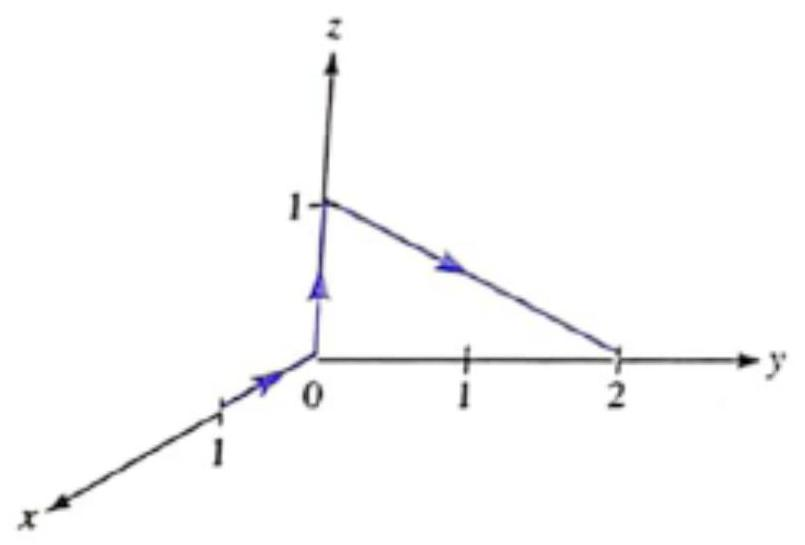
\includegraphics[scale=0.4]{Problemas/2023_02_02_45325701d3410451223eg-3.jpg}
    \end{center}
    \begin{sol}
        Sea
        \begin{align*}
            \int \mathbf{H}\cdot d l &=\left(\int_1+\int_2+\int_3\right)(x-y, x^2+zy,5yz)\cdot dl\\
            \begin{split}
                & = \int_1(x-y, x^2+zy,5yz)\cdot (dx,0,0)+\int_2(x-y, x^2+zy,5yz)\cdot (0,0,dz)+\\
                &+\int_3(x-y, x^2+zy,5yz)\cdot (0,dy,dz)
            \end{split}\\
            \begin{split}
                & = \int_1(x-y)dx+\int_2(5yz)dz+\int_3( (x^2+zy)dy+5yz dz)
            \end{split}\\
            &= \int_1^0(x-y)dx+5y\int_0^1zdz+\int_0^2( (x^2+zy)dy+5yz dz)\\
            &= \int_1^0(x-0)dx+5*0\int_0^1zdz+\int_0^2( (0^2+zy)dy+5yz dz)\\
            &=\int_1^0xdx+\int_0^2\left(-\frac{y}{2}+1\right)ydy+5\int_{0}^2(y)\left(-\frac{y}{2}+1\right) \left(-\frac{dy}{2}\right)\\
            &= \int_1^0xdx+\int_0^2\left(-\frac{y^2}{2}+y\right)dy-\frac{5}{2}\int\left(-\frac{y^2}{2}+y\right) dy\\
            &= 1/2 -2/3 -5/2(-2/3)\\
            &= 3/2
        \end{align*}
    \end{sol}
\end{problema}

\begin{problema}
    

    Find the gradient of the these scalar fields:
    \begin{enumerate}
        \item $U=4 x z^{2}+3 y z$
        \begin{sol}
            Sea
            \begin{align*}
                \nabla &= \left(\frac{\partial U}{\partial x},\frac{\partial U}{\partial y},\frac{\partial U}{\partial z}\right)\\
                &= \left(4z^2, 3z,8xz+3y\right)
            \end{align*}
        \end{sol}
        \item $W=2 \rho\left(z^{2}+1\right) \cos \phi$
        \begin{sol}
            Sea
            \begin{align*}
                \nabla &= \left(\frac{\partial W}{\partial \rho},\frac{1}{\rho }\frac{\partial W}{\partial \phi },\frac{\partial W}{\partial z}\right)\\
                &= \left(2\left(z^{2}+1\right) \cos \phi, -2 \left(z^{2}+1\right) \sin\phi,z\right)
            \end{align*}
        \end{sol}
        \item $H=r^{2} \cos \theta \cos \phi$
        \begin{sol}
            Sea
            \begin{align*}
                \nabla &= \left(\frac{\partial H}{\partial r},\frac{1}{r}\frac{\partial H}{\partial \theta},\frac{1}{r\sin \theta}\frac{\partial H}{\partial \phi}\right)\\
                &= \left(2r \cos \theta \cos \phi,-r \sin \theta \cos \phi,-r \cot \theta \sin \phi\right)
            \end{align*}
        \end{sol}
    \end{enumerate}

\end{problema}

\begin{problema}
    The temperature in an auditorium is given by $T=x^{2}+y^{2}-z$. A mosquito located at $(1,1,2)$ in the auditorium desires to fly in such a direction that it will get warm as soon as possible. In what direction must it fly?
    \begin{sol}
        Sea
        \begin{align*}
            \nabla &= \left(\frac{\partial T}{\partial x},\frac{\partial T}{\partial y},\frac{\partial T}{\partial z}\right)\\
            &= \left(2x,2y,-1\right)
        \end{align*}
        Entonces, en el punto $(1,1,2)$, debe seguir el vector: 
        $$\left(2,2,-1\right)$$
    \end{sol}
\end{problema}

\begin{problema}
    Find the divergence and curl of the following vectors:
    \begin{enumerate}
        \item $\mathbf{A}=e^{x y} \mathbf{a}_{x}+\sin x y \mathbf{a}_{y}+\cos ^{2} x z \mathbf{a}_{z}$
        \begin{sol}
            Sea  5
            \begin{itemize}
                \item Divergencia
                \begin{align*}
                    \nabla\cdot A &= \frac{\partial A_x}{\partial x}+\frac{\partial A_y}{\partial y}+\frac{\partial A_z}{\partial z}\\
                    &= ye^{xy}+x\cos xy-2x\cos zx\sin zxs
                \end{align*}
                \item Rotor
                \begin{align*}
                    \nabla\times A &= \begin{aligned}
                        {\left[\frac{\partial A_z}{\partial y}-\frac{\partial \mathrm{A}_y}{\partial z}\right] \mathbf{a}_x+\left[\frac{\partial A_x}{\partial z}-\frac{\partial \mathrm{A}_z}{\partial x}\right] \mathbf{a}_y}
                        +\left[\frac{\partial A_y}{\partial x}-\frac{\partial \mathrm{A}_x}{\partial y}\right] \mathbf{a}_z
                        \end{aligned}\\
                        &= (0,z2\sin xz,y\cos xy-xe^{xy})
                \end{align*}
            \end{itemize}
        \end{sol}
        \item $\mathbf{B}=\rho z^{2} \cos \phi \mathbf{a}_{p}+z \sin ^{2} \phi \mathbf{a}_{z}$
        \begin{sol}
            Sea 
            \begin{itemize}
                \item Divergencia
                \begin{align*}
                    \nabla\cdot B &= \frac{1}{\rho} \frac{\partial}{\partial \rho}\left(\rho A_\rho\right)+\frac{1}{\rho} \frac{\partial A_\phi}{\partial \phi}+\frac{\partial A_z}{\partial z}\\
                    &=2z^2\cos\phi +\sin^2\phi
                \end{align*}
                \item Rotor
                \begin{align*}
                    \nabla\times B &= \begin{aligned}
                         {\left[\frac{1}{\rho} \frac{\partial A_z}{\partial \phi}-\frac{\partial A_\phi}{\partial z}\right] \mathbf{a}_\rho+\left[\frac{\partial A_\rho}{\partial z}-\frac{\partial A_z}{\partial \rho}\right] \mathbf{a}_\phi}
                         +\frac{1}{\rho}\left[\frac{\partial\left(\rho A_\phi\right)}{\partial \rho}-\frac{\partial A_\rho}{\partial \phi}\right] \mathbf{a}_z
                        \end{aligned}\\
                        &= \left(\frac{z\sin 2\phi}{\rho},2\rho z\cos\phi,z^2\sin \phi\right)
                \end{align*}
            \end{itemize}
        \end{sol}
        \item $\mathbf{C}=r \cos \theta \mathbf{a}_{r}-\frac{1}{r} \sin \theta \mathbf{a}_{\theta}+2 r^{2} \sin \theta \mathbf{a}_{\phi}$ 
        \begin{sol}
            Sea 
            \begin{itemize}
                \item Divergencia
                \begin{align*}
                    \nabla\cdot C &= \frac{1}{r^2} \frac{\partial}{\partial r}\left(r^2 A_r\right)+\frac{1}{r \sin \theta} \frac{\partial}{\partial \theta}\left(A_\theta \sin \theta\right)+\frac{1}{r \sin \theta} \frac{\partial \mathrm{A}_\phi}{\partial \phi}\\
                    &= 3\cos\theta-\frac{2\cos\theta}{r^2}
                \end{align*}
                \item Rotor
                \begin{align*}
                     \nabla\times C &=
                         \frac{1}{r \sin \theta}\left[\frac{\partial\left(A_\phi \sin \theta\right)}{\partial \theta}-\frac{\partial A_\theta}{\partial \phi}\right] \mathbf{a}_r \\
                        & +\frac{1}{r}\left[\frac{1}{\sin \theta} \frac{\partial A_r}{\partial \phi}-\frac{\partial\left(r A_\phi\right)}{\partial r}\right] \mathbf{a}_\theta+\frac{1}{r}\left[\frac{\partial\left(r A_\theta\right)}{\partial r}-\frac{\partial A_r}{\partial \theta}\right] \mathbf{a}_\phi\\
                        &=\left(r\cos\theta,-6r\sin \theta,\sin\theta\right)
                \end{align*}
            \end{itemize}
        \end{sol}
    \end{enumerate}
    
\end{problema}

\begin{problema}

Verify the divergence theorem

$$
\oint_{S} \mathbf{A} \cdot d \mathbf{S}=\int_{v} \nabla \cdot \mathbf{A} d v
$$

for each of the following cases:

\begin{enumerate}
    \item $\mathbf{A}=x y^{2} \mathbf{a}_{x}+y^{3} \mathbf{a}_{y}+y^{2} z \mathbf{a}_{z}$ and $S$ is the surface of the cuboid defined by $0<x<1$, $0<y<1,0<z<1$
    \begin{sol}
        Debemos comprobar los dos lados de la igualdad 
        \begin{itemize}
            \item Sea
            \begin{align*}
                \oint_{S} \mathbf{A} \cdot d \mathbf{S} &= \oint_{S}\left(xy^2,y^3,y^2z\right)\cdot\left(dydz,dxdz,dxdy\right)\\
                &= \oint_{S}\left(xy^2dydz+y^3dxdz+y^2zdxdy\right)\\
                &= \left(\iint_{x=0}+\iint_{x=1}+\iint_{y=0}+\iint_{y=1}+\iint_{z=0}+\iint_{z=1}\right)\\
                &\ \ \ \  \left(xy^2dydz+y^3dxdz+y^2zdxdy\right)\\
                &=x\int_0^1y^2dy \int_{0}^{1}dz+y^3\int_{0}^{1}dx\int_{0}^{1}dz+z\int_0^1y^2dy \int_{0}^{1}dx\\
                &=(1)\left(\frac{(1)^3}{3}\right)+(1)^3+(1)\left(\frac{(1)^3}{3}\right)\\
                &= \frac{1}{3}+1^3+\frac{1}{3} = \frac{5}{3}
            \end{align*}
            \item Sea 
            \begin{align*}
                \int_{v} \nabla \cdot \mathbf{A} d v &=\int_{v} \left(\frac{\partial A_x}{\partial x}+\frac{\partial A_y}{\partial y}+\frac{\partial A_z}{\partial z}\right)dv\\
                &=\int_{v} \left(y^2+3y^2+y^2\right)dxdydz\\
                &=\int_v\left(5y^2\right)dxdydz\\
                &=\int_0^1\int_0^1\int_{0}^{1}\left(5y^2\right)dxdydz\\
                &=\frac{5}{3}(1)^3=\frac{5}{3}
            \end{align*}
        \end{itemize}
        Por lo tanto, se cumple el teorema de la divergencia.
    \end{sol}
    \item $\mathbf{A}=2 \rho z \mathbf{a}_{\rho}+3 z \sin \phi \mathbf{a}_{\phi}-4 \rho \cos \phi \mathbf{a}_{z}$ and $S$ is the surface of the wedge $0<\rho<2$, $0<\phi<45^{\circ}=\pi/4, 0<z<5$
    \begin{sol}
        Debemos comprobar los dos lados de la igualdad 
        \begin{itemize}
            \item Sea
            \begin{align*}
                \oint_{S} \mathbf{A} \cdot d \mathbf{S} &=\oint_{S} \left(2 \rho z ,+3 z \sin \phi ,-4 \rho \cos \phi\right)\cdot \left(\rho d\phi dz,d\rho dz, \rho d\phi d\rho\right)\\
                &= \oint_{S} \left(2 \rho z\rho d\phi dz +3 z \sin \phi d\rho dz -4 \rho \cos \phi \rho d\phi d\rho\right)\\
                &= \left(\iint_{\rho=0}+\iint_{\rho=2}+\iint_{\phi=0}+\iint_{\phi=\pi/4}+\iint_{z=0}+\iint_{z=5}\right)\\
                & \ \ \ \ \left(2 \rho^2 z d\phi dz + 3 z \sin \phi d\rho dz -4 \rho^2 \cos \phi d\phi d\rho\right)\\
                &=\iint_{\rho=2}2 \rho^2 z d\phi dz +\iint_{\phi=\pi/4} 3 z \sin \phi d\rho dz+\\
                & \ \ \ \ \underbrace{-\iint_{z=0}-4 \rho^2 \cos \phi d\phi d\rho+\iint_{z=5}-4 \rho^2 \cos \phi d\phi d\rho}_{\text{se cancelan}}\\
                &= 8\int_{0}^{\pi/4}d\phi \int_0^5 zdz+\frac{3}{\sqrt{2}}\int_{0}^{5}zdz \int_{0}^{2}d\rho \\
                &= 8\left(\frac{\pi}{4}\right)\left(\frac{5^2}{2}\right)+\frac{3}{\sqrt{2}}\left(\frac{5^2}{2}\right)\left(2\right)\\
                &=25\pi +\frac{75}{\sqrt{2}}
            \end{align*}
            \item Sea 
            \begin{align*}
                \int_{v} \nabla \cdot \mathbf{A} d v &=\int_v \left(\frac{1}{\rho} \frac{\partial}{\partial \rho}\left(\rho A_\rho\right)+\frac{1}{\rho} \frac{\partial A_\phi}{\partial \phi}+\frac{\partial A_z}{\partial z}\right)\rho d\rho d\phi dz\\
                &=\int_v \left(\frac{1}{\rho} \frac{\partial}{\partial \rho}\left(2\rho^2z\right)+\frac{1}{\rho} \frac{\partial (3z\sin \phi)}{\partial \phi}+\frac{\partial (-4\rho \cos\phi)}{\partial z}\right)\rho d\rho d\phi dz\\
                &= \int_v \left(4z+\frac{3z\cos\phi}{\rho}+0\right)\rho d\rho d\phi dz\\
                &= \int_v \left(4\rho z+3z\cos\phi\right) d\rho d\phi dz\\
                &= 4\int_{0}^{2}\rho d\rho\int_{0}^{\pi/4}d\phi  \int_0^5 zdz +3\int_{0}^{2}d\rho \int_{0}^{\pi/4}\cos\phi d\phi \int_0^5 zdz\\
                &= 4\left(\frac{2^2}{2}\right)\left(\frac{\pi}{4}\right)\left(\frac{5^2}{2}\right)+3\left(2\right)\left(\sin\left(
                    \frac{\pi}{4}
                \right)\right)\left(\frac{5^2}{2}\right)\\
                &= 25\pi +\frac{150}{2\sqrt{2}}
            \end{align*}
        \end{itemize}
    \end{sol}
    \item $\mathbf{A}=r^{2} \mathbf{a}_{r}+r \sin \theta \cos \phi \mathbf{a}_{\theta}$ and $S$ is the surface of a quarter of a sphere defined by $0<r<3,0<\phi<\pi / 2,0<\theta<\pi / 2$
    \begin{sol}
        Debemos comprobar los dos lados de la igualdad 
        \begin{itemize}
            \item Sea
            \begin{align*}
                \oint_{S} \mathbf{A} \cdot d \mathbf{S} &=\left(\iint_{r=0}+\iint_{r=3}+\iint_{\phi=0}+\iint_{\phi=\pi/2}+\iint_{\theta=0}+\iint_{\theta=\pi/2}\right)\\
                & \ \ \ \ \left(r^2,r\sin\theta\cos\phi,0\right)\cdot (r^2\sin\theta d\theta d\phi,r\sin \theta drd\phi, rdrd\theta)\\
                &= \iint_{r=3}r^4\sin\theta d\theta d\phi+\iint_{\theta=\pi/2}r^2\sin^2\theta\cos\phi drd\phi\\
                &= 3^4\int_0^{\pi/2}\sin\theta d\theta\int_{0}^{\pi/2}d\phi+(1)^2\int_{0}^{3}r^2dr \int_{0}^{\pi/2}\cos\phi d\phi\\
                &= 3^4(-\cos \frac{\pi}{2}+\cos 0)\left(\frac{\pi}{2}\right)+\frac{3^3}{3}\left(\sin\frac{\pi}{2}-\sin 0 \right)\\
                &= \frac{81\pi}{2}+9
            \end{align*}
            \item Sea 
            \begin{align*}
                \int_{v} \nabla \cdot \mathbf{A} d v &=\int_v\left(\frac{1}{r^2}\frac{\partial}{\partial r}(r^2 A_r)+\frac{1}{r\sin\theta}\frac{\partial }{\partial \theta}(A_\theta \sin \theta)+\frac{1}{r\sin \theta}\frac{\partial A_\theta}{\partial \phi}\right)dv\\
                &=\int_v\left(\frac{1}{r^2}\frac{\partial}{\partial r}(r^4)+\frac{1}{r\sin\theta}\frac{\partial }{\partial \theta}(r\sin^2 \theta\cos\phi)+\frac{1}{r\sin \theta}\frac{\partial (0)}{\partial \phi}\right)dv\\
                &=\int_v\left(4r+\frac{r\cos\phi2\sin\theta \cos\theta}{r\sin\theta }\right)dv\\
                &= \int_v\left(4r+2\cos\phi\cos\theta\right)r^2\sin\theta drd\theta d\phi\\
                &= \int_{0}^{3}\int_{0}^{\pi/2}\int_{0}^{\pi/2}\left(4r^3\sin\theta +2r^2\cos\phi \cos\theta\sin\theta\right)drd\theta d\phi\\
                &= 4\int_{0}^{3}r^3dr\int_{0}^{\pi/2}\sin\theta d\theta\int_{0}^{\pi/2}d\phi+2\int_{0}^{3}r^2dr\int_{0}^{\pi/2}\cos\theta\sin\theta d\theta\int_{0}^{\pi/2}\cos\phi d\phi\\
                &= 4\left(\frac{3^4}{4}\right)\left(-\cos\frac{\pi}{2}+\cos 0\right)\left(\frac{\pi}{2}\right)+2\left(\frac{3^3}{3}\right)\left(\frac{1}{2}\right)\left(\sin\frac{\pi}{2}-\sin0\right)\\
                &= 81\left(1\right)\left(\frac{\pi}{2}\right)+9\\
                &=\frac{81\pi }{2}+9
            \end{align*}
        \end{itemize}
    \end{sol}
\end{enumerate}

\end{problema}

\begin{problema}
    Given that $\mathbf{F}=x^{2} y \mathbf{a}_{x}-y \mathbf{a}_{y}$, find

    \begin{enumerate}
        \item $\oint_{L} \mathrm{F} \cdot d \mathrm{l}$ where $L$ is shown in Figure $3.29$.
        \begin{sol}
            Sea 
            \begin{cajita}
                Considerando: 
                \begin{itemize}
                    \item Para (1): $y=x\implies dy=dx$. 
                    \item Para (2): $y=-x+2\implies dy=-dx$
                    \item Para (3): $y=0\implies dy=0$
                \end{itemize}
            \end{cajita}
            \begin{align*}
                \oint_{L} \mathrm{F} \cdot d \mathrm{l} &= \oint_L \left(x^2y,-y,0\right)\cdot \left(dx,dy,dz\right)\\
                &=\left(\int_1+\int_2+\int_3\right) \left(x^2ydx -ydy\right)\\
                &= \int_1(x^2ydx -ydy) + \int_2(x^2ydx -ydy)+\int_3(x^2ydx -ydy)\\
                &= \int_1(x^2(x)dx -xdx) + \int_2(x^2(-x+2)dx -(-x+2)(-dx))+0\\
                &= \int_0^1(x^3-x)dx + \int_1^2\left(-x^3+2x^2 -x+2\right)dx\\
                &= \frac{(1)^4}{4}-\frac{1^2}{2}+\left(\frac{17}{12}\right)\\
                &= \frac{7}{6}
            \end{align*}
        \end{sol}

        \item $\int_{S}(\nabla \times \mathbf{F}) \cdot d S$ where $S$ is the area bounded by $L$.
        \begin{sol}
            Sea
            \begin{align*}
                \int_{S}(\nabla \times \mathbf{F}) \cdot d S &= \left(\iint_1+\iint_2+\iint_3\right)\\
                & \ \ \ \left(\frac{\partial A_z}{\partial y}-\frac{\partial \mathrm{A}_y}{\partial z},\frac{\partial A_x}{\partial z}-\frac{\partial \mathrm{A}_z}{\partial x},
                    \frac{\partial A_y}{\partial x}-\frac{\partial \mathrm{A}_x}{\partial y}\right) \cdot \left(dydx,dxdz,-dxdy\right)\\
                    &=\left(\iint_1+\iint_2+\iint_3\right) \left(0-0,0-0,0-x^2\right) \cdot \left(dydx,dxdz,-dxdy\right)\\
                    &=\left(\iint_1+\iint_2+\iint_3\right) \left(x^2dxdy\right)\\
                    &=\iint_1\left(x^2dxdy\right) +\iint_2\left(x^2dxdy\right)+\iint_3\left(x^2dxdy\right)\\
                    &=\int_0^1 x^2dx \int_{0}^{x} dy +\int_{1}^{2}x^2dx\int_{0}^{-x+2} dy+0\\
                    &=\int_0^1 x^2(x)dx +\int_{1}^{2}x^2(-x+2)dx\\
                    &=\frac{7}{6}
            \end{align*}

        \end{sol}
        \item  Is Stokes's theorem satisfied?
        \begin{sol}
            Sí, se cumple la igualdad. 
        \end{sol}
    \end{enumerate}



\begin{center}
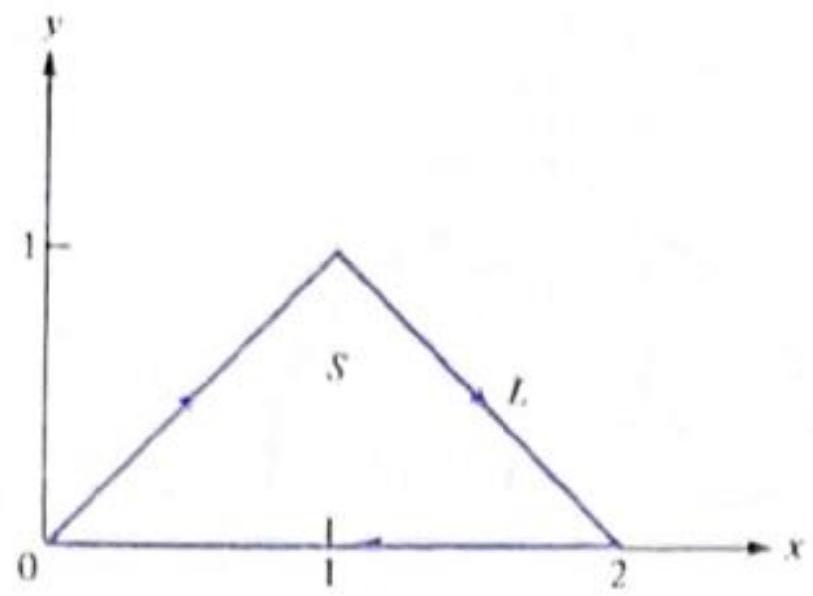
\includegraphics[scale=0.4]{Problemas/2023_02_02_45325701d3410451223eg-5}
\end{center}
\end{problema}

\begin{problema}

Given the vector field

$$
\mathbf{G}=(16 x y-z) \mathrm{a}_{x}+8 x^{2} \mathrm{a}_{y}-x \mathrm{a}_{z}
$$
Assume anticlockwise direction.

\begin{enumerate}
    \item Is $\mathbf{G}$ irrotational (or conservative)?
        \begin{sol}
            Es necesario determinar si se cumple o no: $\nabla \times G=0$.
            \begin{align*}
                \nabla \times G &= \left(\frac{\partial A_z}{\partial y}-\frac{\partial \mathrm{A}_y}{\partial z},\frac{\partial A_x}{\partial z}-\frac{\partial \mathrm{A}_z}{\partial x},
                \frac{\partial A_y}{\partial x}-\frac{\partial \mathrm{A}_x}{\partial y}\right)\\
                &=(0,0,0)
            \end{align*}
            Entonces es irrotacional.
        \end{sol}
    \item Find the net flux of $\mathbf{G}$ over the cube $0<x, y, z<1$.
    \begin{sol}
        Sea 
        \begin{align*}
            \oint G \cdot d S&=\int \nabla \cdot G d v\\
            &= \iiint 16 y d x d y d z=16 \int_0^1 d x \int_0^1 d z \int_0^1 y d y\\
            &= 8
        \end{align*}
        
    \end{sol}
    
    \item Determine the circulation of $\mathbf{G}$ around the edge of the square $z=0,0<x, y<1$.
    \begin{sol}
        Sea
        \begin{align*}
            \oint G\cdot dl &=\left(\int_1 +\int_2 +\int_3 +\int_4\right)(16xy-z,8x^2,-x)\cdot (dx,dy,-dz)\\
            &=\left(\int_{x=0,z=0} +\int_{y=1,z=0} +\int_{x=1,z=0} +\int_{y=0,z=0}\right)((16xy-z)dx+(8x^2)dy+xdz)\\
            &=\int_{y=1,z=0}((16xy-z)dx+(8x^2)dy+xdz)\\ & \ \ +\int_{x=1,z=0}((16xy-z)dx+(8x^2)dy+xdz)\\
            &= 16\int_0^1 xdx+8\int_1^0 dy\\
            &= 16\left(\frac{1}{2}\right)-8\\
            &= 0
        \end{align*}
    \end{sol}
\end{enumerate}



\end{problema}
%---------------------------
%\bibliographystyle{apa}
%\bibliography{referencias.bib}

\end{document}